% ------------------------------------------------
\StartChapter{各系所博碩士撰寫論文須知}{appendix:thesis-spec}
% ------------------------------------------------

\section{介紹}
這部份資料來源是使用'電機工程系辦網頁'中的'論文撰寫須知.pdf'\cite{web:ncku:thesis-need-to-know}.\\

但由於原檔案沒法顯示, 故需要另重新儲存成一個新的出來. 使用學校的Adobe Acrobat XI試驗, 發現要使用'儲存為其他->可存檔PDF (PDF/A)'才能顯示出來.\\

\InsertCenterImage
  [scale=0.3,
    caption={在Adobe Acrobat另存新版本},
    label={fig:appendix:save_pdf}]
  {./example/appendix/pic/save_pdf.png}

\noindent 檔案位置:\\
\noindent 新: 'example/appendix/pdf/thesis-spec.pdf'\\
\noindent 原: 'example/appendix/pdf/論文撰寫須知.pdf'\\

\setboolean{@twoside}{false}
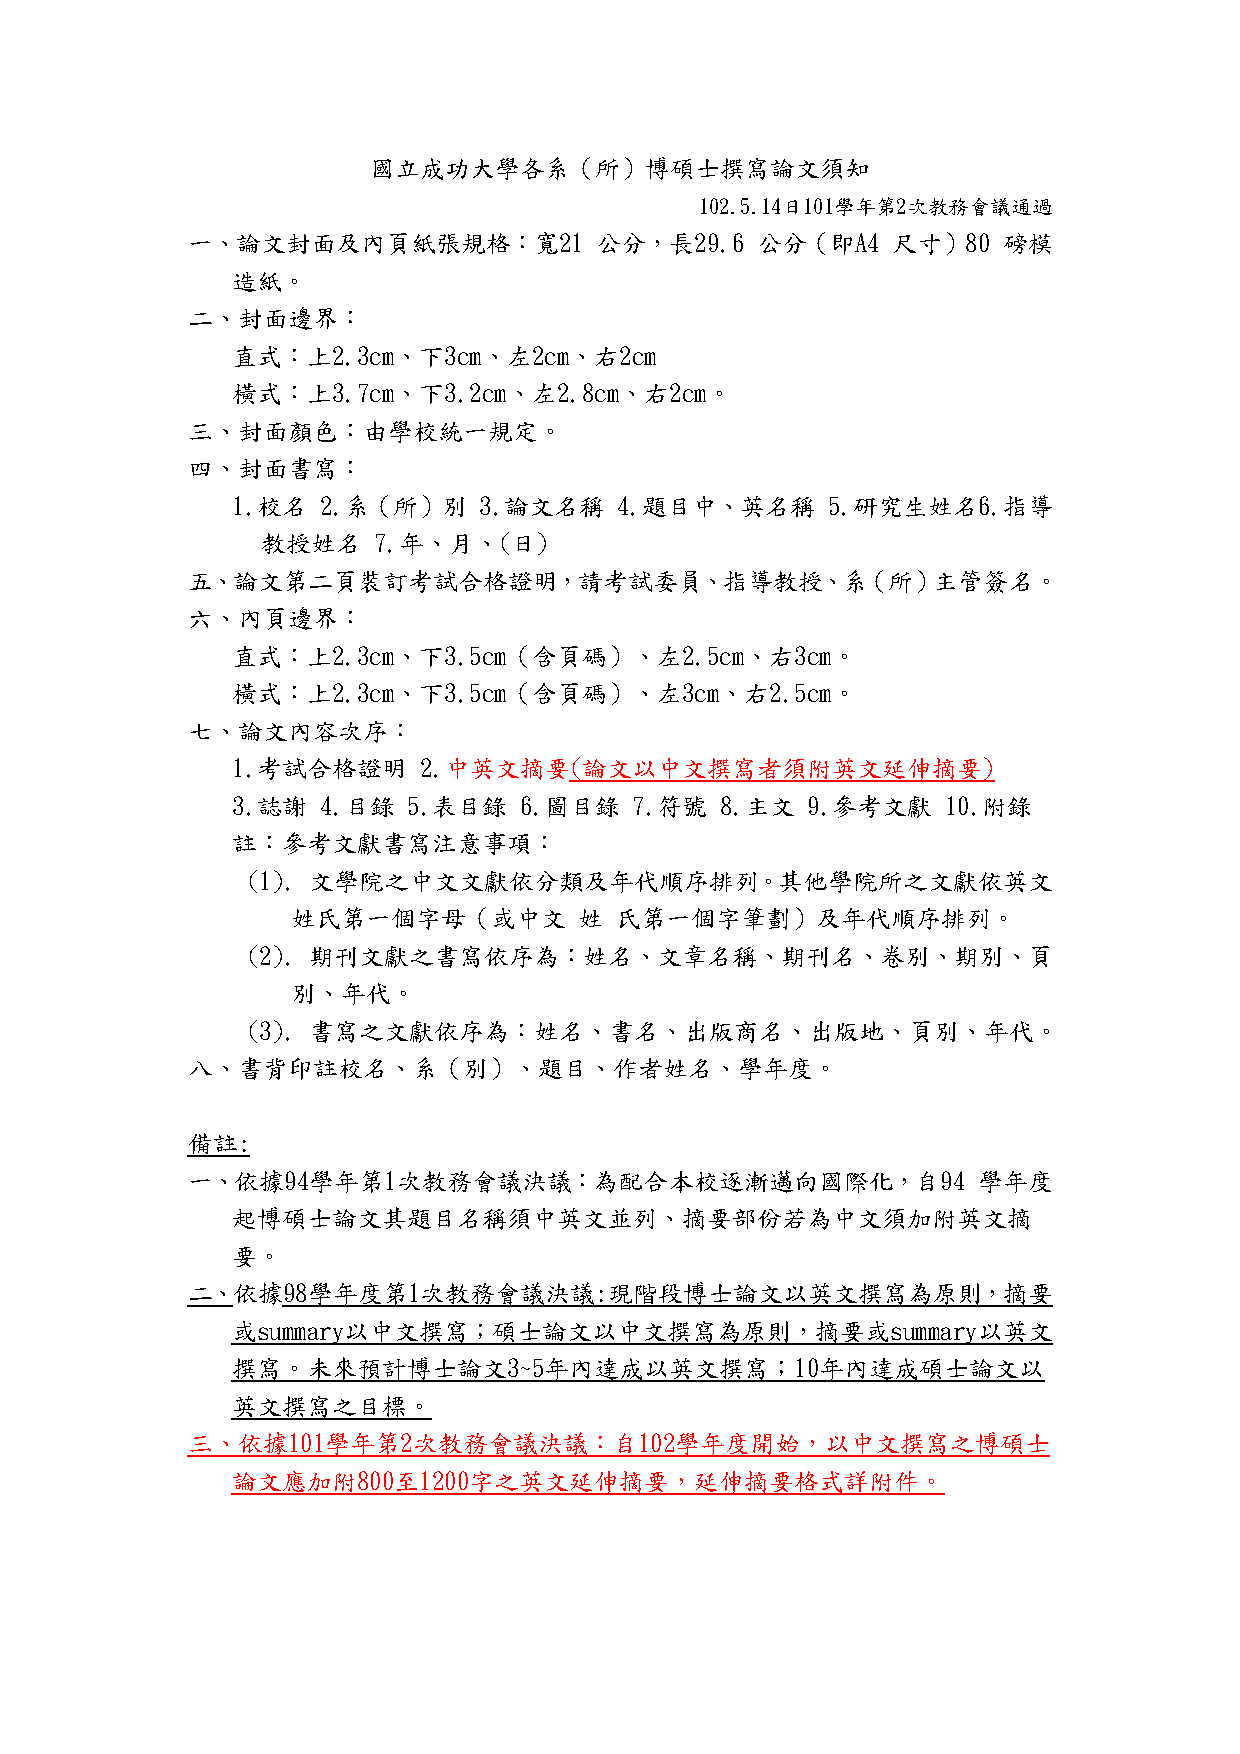
\includepdf[pages=-]{./example/appendix/pdf/thesis-spec.pdf}

% ------------------------------------------------
\EndChapter
% ------------------------------------------------
